\documentclass[a4paper,11pt,final]{article}
        \usepackage{fancyvrb, color, graphicx, hyperref, ,amsmath, url}
        \usepackage{palatino}
        \usepackage[a4paper,text={16.5cm,25.2cm},centering]{geometry}

        \hypersetup
        {   pdfauthor = {Pweave},
            pdftitle={Published from BIOE232_HW19.py},
            colorlinks=TRUE,
            linkcolor=black,
            citecolor=blue,
            urlcolor=blue
        }
        \setlength{\parindent}{0pt}
        \setlength{\parskip}{1.2ex}
        
\makeatletter
\def\PY@reset{\let\PY@it=\relax \let\PY@bf=\relax%
    \let\PY@ul=\relax \let\PY@tc=\relax%
    \let\PY@bc=\relax \let\PY@ff=\relax}
\def\PY@tok#1{\csname PY@tok@#1\endcsname}
\def\PY@toks#1+{\ifx\relax#1\empty\else%
    \PY@tok{#1}\expandafter\PY@toks\fi}
\def\PY@do#1{\PY@bc{\PY@tc{\PY@ul{%
    \PY@it{\PY@bf{\PY@ff{#1}}}}}}}
\def\PY#1#2{\PY@reset\PY@toks#1+\relax+\PY@do{#2}}

\expandafter\def\csname PY@tok@gd\endcsname{\def\PY@tc##1{\textcolor[rgb]{0.63,0.00,0.00}{##1}}}
\expandafter\def\csname PY@tok@gu\endcsname{\let\PY@bf=\textbf\def\PY@tc##1{\textcolor[rgb]{0.50,0.00,0.50}{##1}}}
\expandafter\def\csname PY@tok@gt\endcsname{\def\PY@tc##1{\textcolor[rgb]{0.00,0.27,0.87}{##1}}}
\expandafter\def\csname PY@tok@gs\endcsname{\let\PY@bf=\textbf}
\expandafter\def\csname PY@tok@gr\endcsname{\def\PY@tc##1{\textcolor[rgb]{1.00,0.00,0.00}{##1}}}
\expandafter\def\csname PY@tok@cm\endcsname{\let\PY@it=\textit\def\PY@tc##1{\textcolor[rgb]{0.25,0.50,0.50}{##1}}}
\expandafter\def\csname PY@tok@vg\endcsname{\def\PY@tc##1{\textcolor[rgb]{0.10,0.09,0.49}{##1}}}
\expandafter\def\csname PY@tok@m\endcsname{\def\PY@tc##1{\textcolor[rgb]{0.40,0.40,0.40}{##1}}}
\expandafter\def\csname PY@tok@mh\endcsname{\def\PY@tc##1{\textcolor[rgb]{0.40,0.40,0.40}{##1}}}
\expandafter\def\csname PY@tok@go\endcsname{\def\PY@tc##1{\textcolor[rgb]{0.53,0.53,0.53}{##1}}}
\expandafter\def\csname PY@tok@ge\endcsname{\let\PY@it=\textit}
\expandafter\def\csname PY@tok@vc\endcsname{\def\PY@tc##1{\textcolor[rgb]{0.10,0.09,0.49}{##1}}}
\expandafter\def\csname PY@tok@il\endcsname{\def\PY@tc##1{\textcolor[rgb]{0.40,0.40,0.40}{##1}}}
\expandafter\def\csname PY@tok@cs\endcsname{\let\PY@it=\textit\def\PY@tc##1{\textcolor[rgb]{0.25,0.50,0.50}{##1}}}
\expandafter\def\csname PY@tok@cp\endcsname{\def\PY@tc##1{\textcolor[rgb]{0.74,0.48,0.00}{##1}}}
\expandafter\def\csname PY@tok@gi\endcsname{\def\PY@tc##1{\textcolor[rgb]{0.00,0.63,0.00}{##1}}}
\expandafter\def\csname PY@tok@gh\endcsname{\let\PY@bf=\textbf\def\PY@tc##1{\textcolor[rgb]{0.00,0.00,0.50}{##1}}}
\expandafter\def\csname PY@tok@ni\endcsname{\let\PY@bf=\textbf\def\PY@tc##1{\textcolor[rgb]{0.60,0.60,0.60}{##1}}}
\expandafter\def\csname PY@tok@nl\endcsname{\def\PY@tc##1{\textcolor[rgb]{0.63,0.63,0.00}{##1}}}
\expandafter\def\csname PY@tok@nn\endcsname{\let\PY@bf=\textbf\def\PY@tc##1{\textcolor[rgb]{0.00,0.00,1.00}{##1}}}
\expandafter\def\csname PY@tok@no\endcsname{\def\PY@tc##1{\textcolor[rgb]{0.53,0.00,0.00}{##1}}}
\expandafter\def\csname PY@tok@na\endcsname{\def\PY@tc##1{\textcolor[rgb]{0.49,0.56,0.16}{##1}}}
\expandafter\def\csname PY@tok@nb\endcsname{\def\PY@tc##1{\textcolor[rgb]{0.00,0.50,0.00}{##1}}}
\expandafter\def\csname PY@tok@nc\endcsname{\let\PY@bf=\textbf\def\PY@tc##1{\textcolor[rgb]{0.00,0.00,1.00}{##1}}}
\expandafter\def\csname PY@tok@nd\endcsname{\def\PY@tc##1{\textcolor[rgb]{0.67,0.13,1.00}{##1}}}
\expandafter\def\csname PY@tok@ne\endcsname{\let\PY@bf=\textbf\def\PY@tc##1{\textcolor[rgb]{0.82,0.25,0.23}{##1}}}
\expandafter\def\csname PY@tok@nf\endcsname{\def\PY@tc##1{\textcolor[rgb]{0.00,0.00,1.00}{##1}}}
\expandafter\def\csname PY@tok@si\endcsname{\let\PY@bf=\textbf\def\PY@tc##1{\textcolor[rgb]{0.73,0.40,0.53}{##1}}}
\expandafter\def\csname PY@tok@s2\endcsname{\def\PY@tc##1{\textcolor[rgb]{0.73,0.13,0.13}{##1}}}
\expandafter\def\csname PY@tok@vi\endcsname{\def\PY@tc##1{\textcolor[rgb]{0.10,0.09,0.49}{##1}}}
\expandafter\def\csname PY@tok@nt\endcsname{\let\PY@bf=\textbf\def\PY@tc##1{\textcolor[rgb]{0.00,0.50,0.00}{##1}}}
\expandafter\def\csname PY@tok@nv\endcsname{\def\PY@tc##1{\textcolor[rgb]{0.10,0.09,0.49}{##1}}}
\expandafter\def\csname PY@tok@s1\endcsname{\def\PY@tc##1{\textcolor[rgb]{0.73,0.13,0.13}{##1}}}
\expandafter\def\csname PY@tok@kd\endcsname{\let\PY@bf=\textbf\def\PY@tc##1{\textcolor[rgb]{0.00,0.50,0.00}{##1}}}
\expandafter\def\csname PY@tok@sh\endcsname{\def\PY@tc##1{\textcolor[rgb]{0.73,0.13,0.13}{##1}}}
\expandafter\def\csname PY@tok@sc\endcsname{\def\PY@tc##1{\textcolor[rgb]{0.73,0.13,0.13}{##1}}}
\expandafter\def\csname PY@tok@sx\endcsname{\def\PY@tc##1{\textcolor[rgb]{0.00,0.50,0.00}{##1}}}
\expandafter\def\csname PY@tok@bp\endcsname{\def\PY@tc##1{\textcolor[rgb]{0.00,0.50,0.00}{##1}}}
\expandafter\def\csname PY@tok@c1\endcsname{\let\PY@it=\textit\def\PY@tc##1{\textcolor[rgb]{0.25,0.50,0.50}{##1}}}
\expandafter\def\csname PY@tok@kc\endcsname{\let\PY@bf=\textbf\def\PY@tc##1{\textcolor[rgb]{0.00,0.50,0.00}{##1}}}
\expandafter\def\csname PY@tok@c\endcsname{\let\PY@it=\textit\def\PY@tc##1{\textcolor[rgb]{0.25,0.50,0.50}{##1}}}
\expandafter\def\csname PY@tok@mf\endcsname{\def\PY@tc##1{\textcolor[rgb]{0.40,0.40,0.40}{##1}}}
\expandafter\def\csname PY@tok@err\endcsname{\def\PY@bc##1{\setlength{\fboxsep}{0pt}\fcolorbox[rgb]{1.00,0.00,0.00}{1,1,1}{\strut ##1}}}
\expandafter\def\csname PY@tok@mb\endcsname{\def\PY@tc##1{\textcolor[rgb]{0.40,0.40,0.40}{##1}}}
\expandafter\def\csname PY@tok@ss\endcsname{\def\PY@tc##1{\textcolor[rgb]{0.10,0.09,0.49}{##1}}}
\expandafter\def\csname PY@tok@sr\endcsname{\def\PY@tc##1{\textcolor[rgb]{0.73,0.40,0.53}{##1}}}
\expandafter\def\csname PY@tok@mo\endcsname{\def\PY@tc##1{\textcolor[rgb]{0.40,0.40,0.40}{##1}}}
\expandafter\def\csname PY@tok@kn\endcsname{\let\PY@bf=\textbf\def\PY@tc##1{\textcolor[rgb]{0.00,0.50,0.00}{##1}}}
\expandafter\def\csname PY@tok@mi\endcsname{\def\PY@tc##1{\textcolor[rgb]{0.40,0.40,0.40}{##1}}}
\expandafter\def\csname PY@tok@gp\endcsname{\let\PY@bf=\textbf\def\PY@tc##1{\textcolor[rgb]{0.00,0.00,0.50}{##1}}}
\expandafter\def\csname PY@tok@o\endcsname{\def\PY@tc##1{\textcolor[rgb]{0.40,0.40,0.40}{##1}}}
\expandafter\def\csname PY@tok@kr\endcsname{\let\PY@bf=\textbf\def\PY@tc##1{\textcolor[rgb]{0.00,0.50,0.00}{##1}}}
\expandafter\def\csname PY@tok@s\endcsname{\def\PY@tc##1{\textcolor[rgb]{0.73,0.13,0.13}{##1}}}
\expandafter\def\csname PY@tok@kp\endcsname{\def\PY@tc##1{\textcolor[rgb]{0.00,0.50,0.00}{##1}}}
\expandafter\def\csname PY@tok@w\endcsname{\def\PY@tc##1{\textcolor[rgb]{0.73,0.73,0.73}{##1}}}
\expandafter\def\csname PY@tok@kt\endcsname{\def\PY@tc##1{\textcolor[rgb]{0.69,0.00,0.25}{##1}}}
\expandafter\def\csname PY@tok@ow\endcsname{\let\PY@bf=\textbf\def\PY@tc##1{\textcolor[rgb]{0.67,0.13,1.00}{##1}}}
\expandafter\def\csname PY@tok@sb\endcsname{\def\PY@tc##1{\textcolor[rgb]{0.73,0.13,0.13}{##1}}}
\expandafter\def\csname PY@tok@k\endcsname{\let\PY@bf=\textbf\def\PY@tc##1{\textcolor[rgb]{0.00,0.50,0.00}{##1}}}
\expandafter\def\csname PY@tok@se\endcsname{\let\PY@bf=\textbf\def\PY@tc##1{\textcolor[rgb]{0.73,0.40,0.13}{##1}}}
\expandafter\def\csname PY@tok@sd\endcsname{\let\PY@it=\textit\def\PY@tc##1{\textcolor[rgb]{0.73,0.13,0.13}{##1}}}

\def\PYZbs{\char`\\}
\def\PYZus{\char`\_}
\def\PYZob{\char`\{}
\def\PYZcb{\char`\}}
\def\PYZca{\char`\^}
\def\PYZam{\char`\&}
\def\PYZlt{\char`\<}
\def\PYZgt{\char`\>}
\def\PYZsh{\char`\#}
\def\PYZpc{\char`\%}
\def\PYZdl{\char`\$}
\def\PYZhy{\char`\-}
\def\PYZsq{\char`\'}
\def\PYZdq{\char`\"}
\def\PYZti{\char`\~}
% for compatibility with earlier versions
\def\PYZat{@}
\def\PYZlb{[}
\def\PYZrb{]}
\makeatother

        
\title{ HW19 - BIOE232}
\author{ Kyle King}
\date{ May 7, 2015}

\begin{document}
\maketitle
My First Python Script!

\begin{Verbatim}[commandchars=\\\{\},frame=single,fontsize=\small, xleftmargin=0.5em]
\PY{c}{\PYZsh{} For outputting nice HTML file/PDF}
\PY{c}{\PYZsh{} import pweave}
\PY{k+kn}{import} \PY{n+nn}{pprint} \PY{k+kn}{as} \PY{n+nn}{pp}

\PY{c}{\PYZsh{} All the essentials}
\PY{k+kn}{import} \PY{n+nn}{numpy} \PY{k+kn}{as} \PY{n+nn}{np}  \PY{c}{\PYZsh{} np.\PYZus{}\PYZus{}version\PYZus{}\PYZus{}}
\PY{k+kn}{import} \PY{n+nn}{matplotlib.pyplot} \PY{k+kn}{as} \PY{n+nn}{plt}
\PY{k+kn}{import} \PY{n+nn}{math}
\PY{k+kn}{from} \PY{n+nn}{decimal} \PY{k+kn}{import} \PY{o}{*}
\PY{k+kn}{from} \PY{n+nn}{pylab} \PY{k+kn}{import} \PY{o}{*}
\end{Verbatim}

Question 1

\begin{Verbatim}[commandchars=\\\{\},frame=single,fontsize=\small, xleftmargin=0.5em]
\PY{c}{\PYZsh{} Declare varibales}
\PY{n}{Ka} \PY{o}{=} \PY{l+m+mf}{5.1E\PYZhy{}7}
\PY{n}{pKa} \PY{o}{=} \PY{o}{\PYZhy{}}\PY{n}{math}\PY{o}{.}\PY{n}{log10}\PY{p}{(}\PY{n}{Ka}\PY{p}{)}
\PY{n}{pH} \PY{o}{=} \PY{n}{np}\PY{o}{.}\PY{n}{linspace}\PY{p}{(}\PY{l+m+mi}{0}\PY{p}{,} \PY{l+m+mi}{14}\PY{p}{,} \PY{n}{num}\PY{o}{=}\PY{l+m+mi}{140}\PY{p}{)}
\PY{n}{ratio} \PY{o}{=} \PY{l+m+mi}{1}\PY{o}{/}\PY{p}{(}\PY{l+m+mi}{1} \PY{o}{+} \PY{n+nb}{pow}\PY{p}{(}\PY{l+m+mi}{10}\PY{p}{,} \PY{p}{(}\PY{n}{pKa} \PY{o}{\PYZhy{}} \PY{n}{pH}\PY{p}{)}\PY{p}{)}\PY{p}{)}

\PY{c}{\PYZsh{} Print out constants}
\PY{n}{pp}\PY{o}{.}\PY{n}{pprint}\PY{p}{(}\PY{p}{[}\PY{l+s}{\PYZsq{}}\PY{l+s}{Ka = }\PY{l+s}{\PYZsq{}}\PY{p}{,} \PY{n}{Ka}\PY{p}{]}\PY{p}{)}
\PY{n}{pp}\PY{o}{.}\PY{n}{pprint}\PY{p}{(}\PY{p}{[}\PY{l+s}{\PYZsq{}}\PY{l+s}{pKa = }\PY{l+s}{\PYZsq{}}\PY{p}{,} \PY{n}{pKa}\PY{p}{]}\PY{p}{)}

\PY{c}{\PYZsh{} Plot function}
\PY{n}{plot}\PY{p}{(}\PY{n}{pH}\PY{p}{,} \PY{n}{ratio}\PY{p}{)}
\PY{n}{title}\PY{p}{(}\PY{l+s}{\PYZsq{}}\PY{l+s}{HW19: Q1 The ratio of C\PYZus{}b / C\PYZus{}total versus pH}\PY{l+s}{\PYZsq{}}\PY{p}{)}
\PY{n}{xlabel}\PY{p}{(}\PY{l+s}{\PYZsq{}}\PY{l+s}{pH}\PY{l+s}{\PYZsq{}}\PY{p}{)}
\PY{n}{ylabel}\PY{p}{(}\PY{l+s}{\PYZsq{}}\PY{l+s}{Ratio of C\PYZus{}b / C\PYZus{}total}\PY{l+s}{\PYZsq{}}\PY{p}{)}
\PY{n}{grid}\PY{p}{(}\PY{n+nb+bp}{True}\PY{p}{)}
\PY{c}{\PYZsh{} show()}
\end{Verbatim}
\begin{Verbatim}[commandchars=\\\{\},frame=leftline,fontsize=\small, xleftmargin=0.5em]
[\PYZsq{}Ka = \PYZsq{}, 5.1e\PYZhy{}07]
[\PYZsq{}pKa = \PYZsq{}, 6.292429823902063]
\end{Verbatim}
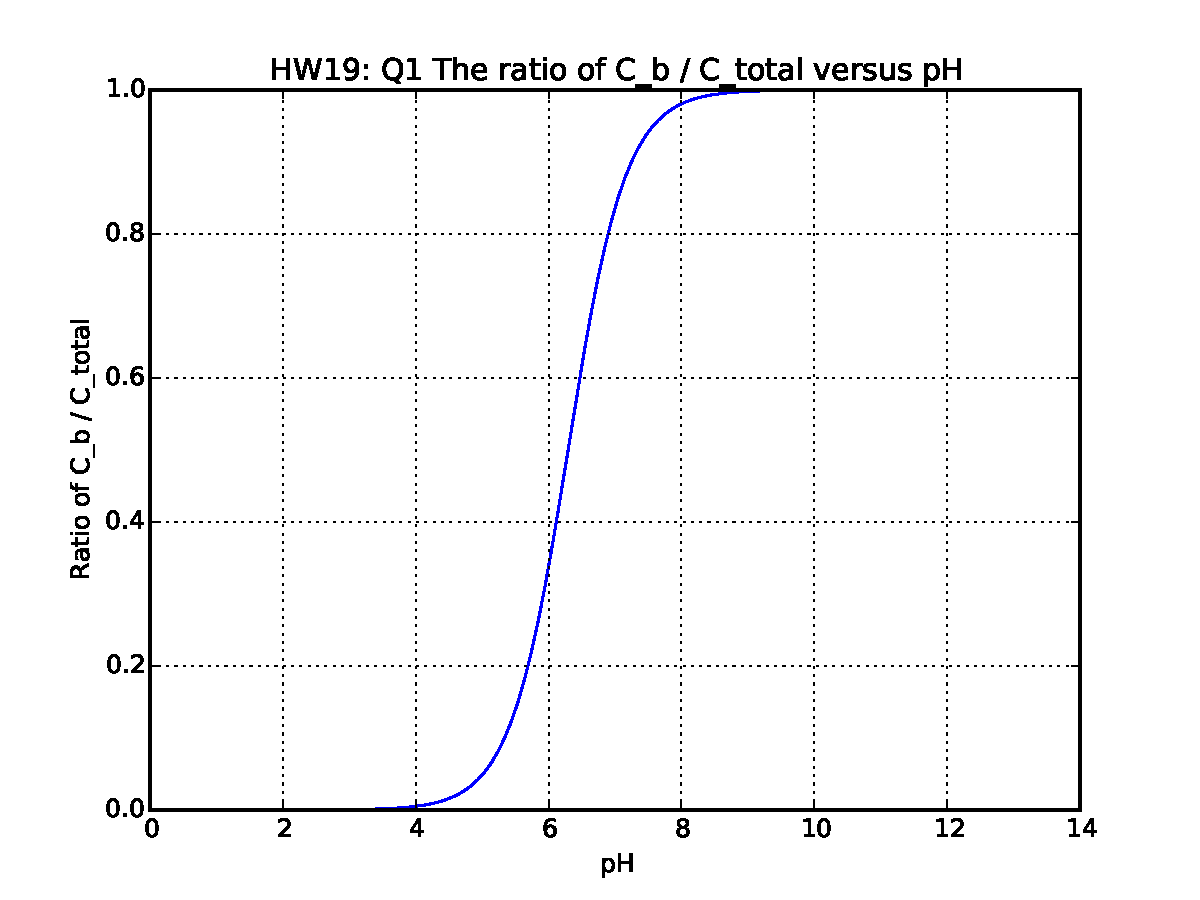
\includegraphics[width= \linewidth]{figures/BIOE232_HW19_figure3_1.pdf}

Question 2

\begin{Verbatim}[commandchars=\\\{\},frame=single,fontsize=\small, xleftmargin=0.5em]
\PY{c}{\PYZsh{} Declare varibales}
\PY{n}{pKa1}\PY{p}{,} \PY{n}{pKa2} \PY{o}{=} \PY{l+m+mf}{6.3}\PY{p}{,} \PY{l+m+mf}{10.8}
\PY{n}{pH} \PY{o}{=} \PY{n}{np}\PY{o}{.}\PY{n}{linspace}\PY{p}{(}\PY{l+m+mi}{0}\PY{p}{,} \PY{l+m+mi}{14}\PY{p}{,} \PY{n}{num}\PY{o}{=}\PY{l+m+mi}{140}\PY{p}{)}
\PY{n}{Dratio1} \PY{o}{=} \PY{l+m+mi}{1}\PY{o}{/}\PY{p}{(}\PY{l+m+mi}{1} \PY{o}{+} \PY{n+nb}{pow}\PY{p}{(}\PY{l+m+mi}{10}\PY{p}{,} \PY{p}{(}\PY{n}{pKa1} \PY{o}{\PYZhy{}} \PY{n}{pH}\PY{p}{)}\PY{p}{)}\PY{p}{)}
\PY{n}{Dratio2} \PY{o}{=} \PY{l+m+mi}{1}\PY{o}{/}\PY{p}{(}\PY{l+m+mi}{1} \PY{o}{+} \PY{n+nb}{pow}\PY{p}{(}\PY{l+m+mi}{10}\PY{p}{,} \PY{p}{(}\PY{n}{pKa2} \PY{o}{\PYZhy{}} \PY{n}{pH}\PY{p}{)}\PY{p}{)}\PY{p}{)}

\PY{c}{\PYZsh{} Print out constants}
\PY{c}{\PYZsh{} pp.pprint([\PYZsq{}Dratio1 = \PYZsq{}, Dratio1])}
\PY{c}{\PYZsh{} pp.pprint([\PYZsq{}Dratio2 = \PYZsq{}, Dratio2])}

\PY{c}{\PYZsh{} Plot function}
\PY{n}{fig} \PY{o}{=} \PY{n}{plt}\PY{o}{.}\PY{n}{figure}\PY{p}{(}\PY{p}{)}
\PY{n}{ax1} \PY{o}{=} \PY{n}{fig}\PY{o}{.}\PY{n}{add\PYZus{}axes}\PY{p}{(}\PY{p}{[}\PY{l+m+mf}{0.1}\PY{p}{,} \PY{l+m+mf}{0.1}\PY{p}{,} \PY{l+m+mf}{0.8}\PY{p}{,} \PY{l+m+mf}{0.7}\PY{p}{]}\PY{p}{)}
\PY{n}{l1}\PY{p}{,} \PY{n}{l2} \PY{o}{=} \PY{n}{ax1}\PY{o}{.}\PY{n}{plot}\PY{p}{(}\PY{n}{pH}\PY{p}{,} \PY{n}{Dratio1}\PY{p}{,} \PY{l+s}{\PYZsq{}}\PY{l+s}{\PYZhy{}*}\PY{l+s}{\PYZsq{}}\PY{p}{,} \PY{n}{pH}\PY{p}{,} \PY{n}{Dratio2}\PY{p}{)}
\PY{n}{fig}\PY{o}{.}\PY{n}{legend}\PY{p}{(}\PY{p}{(}\PY{n}{l1}\PY{p}{,} \PY{n}{l2}\PY{p}{)}\PY{p}{,} \PY{p}{(}\PY{l+s}{\PYZsq{}}\PY{l+s}{Ajmalicine}\PY{l+s}{\PYZsq{}}\PY{p}{,} \PY{l+s}{\PYZsq{}}\PY{l+s}{Serpentine}\PY{l+s}{\PYZsq{}}\PY{p}{)}\PY{p}{,} \PY{l+s}{\PYZsq{}}\PY{l+s}{upper right}\PY{l+s}{\PYZsq{}}\PY{p}{)}
\PY{n}{title}\PY{p}{(}\PY{l+s}{\PYZsq{}}\PY{l+s}{HW19: Q2 The ratio of D\PYZus{}overall / D versus pH}\PY{l+s}{\PYZsq{}}\PY{p}{)}
\PY{n}{xlabel}\PY{p}{(}\PY{l+s}{\PYZsq{}}\PY{l+s}{pH}\PY{l+s}{\PYZsq{}}\PY{p}{)}
\PY{n}{ylabel}\PY{p}{(}\PY{l+s}{\PYZsq{}}\PY{l+s}{Ratio of D\PYZus{}overall / D}\PY{l+s}{\PYZsq{}}\PY{p}{)}
\PY{n}{grid}\PY{p}{(}\PY{n+nb+bp}{True}\PY{p}{)}
\PY{c}{\PYZsh{} plt.show()}
\end{Verbatim}
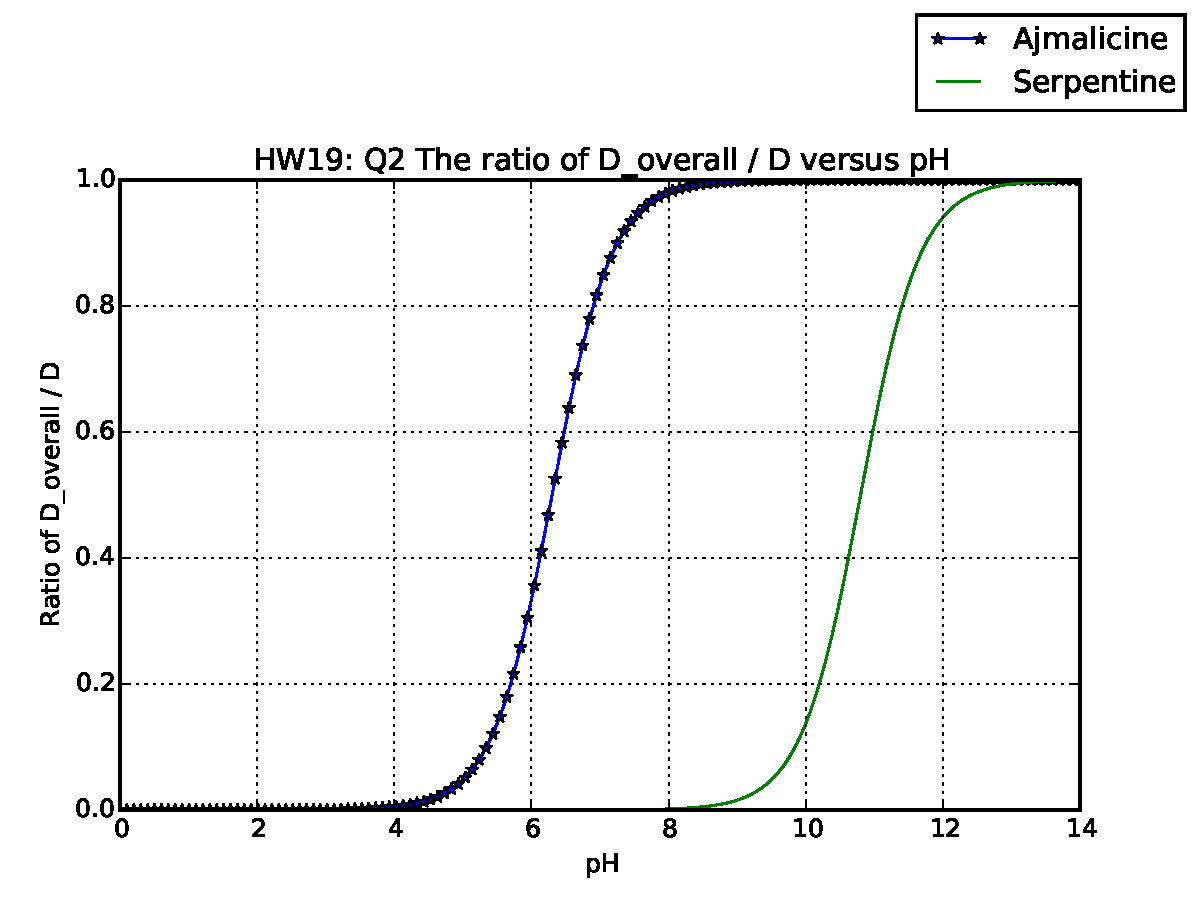
\includegraphics[width= \linewidth]{figures/BIOE232_HW19_figure4_1.pdf}

Question 3

\begin{Verbatim}[commandchars=\\\{\},frame=single,fontsize=\small, xleftmargin=0.5em]
\PY{n}{pKa}\PY{p}{,} \PY{n}{pHv}\PY{p}{,} \PY{n}{pHc} \PY{o}{=} \PY{l+m+mf}{6.3}\PY{p}{,} \PY{l+m+mi}{3}\PY{p}{,} \PY{l+m+mi}{7}

\PY{n}{conc} \PY{o}{=} \PY{p}{(}\PY{l+m+mi}{1}\PY{o}{+}\PY{n+nb}{pow}\PY{p}{(}\PY{l+m+mi}{10}\PY{p}{,} \PY{n}{pKa} \PY{o}{\PYZhy{}} \PY{n}{pHv}\PY{p}{)}\PY{p}{)} \PY{o}{/} \PY{p}{(}\PY{l+m+mi}{1}\PY{o}{+}\PY{n+nb}{pow}\PY{p}{(}\PY{l+m+mi}{10}\PY{p}{,} \PY{n}{pKa} \PY{o}{\PYZhy{}} \PY{n}{pHc}\PY{p}{)}\PY{p}{)}
\PY{n}{pp}\PY{o}{.}\PY{n}{pprint}\PY{p}{(}\PY{p}{[}\PY{l+s}{\PYZsq{}}\PY{l+s}{Concentration Ability = }\PY{l+s}{\PYZsq{}}\PY{p}{,} \PY{n}{conc}\PY{p}{]}\PY{p}{)}
\end{Verbatim}
\begin{Verbatim}[commandchars=\\\{\},frame=leftline,fontsize=\small, xleftmargin=0.5em]
[\PYZsq{}Concentration Ability = \PYZsq{}, 1664.2089706348017]
\end{Verbatim}
\end{document}